\documentclass[a4paper]{article}
\usepackage{latexsym}
\usepackage[a4paper]{geometry}
\usepackage{color}
\usepackage{listings}
\usepackage[pdftex]{graphicx}
\usepackage{subfig}

\definecolor{Blue}{rgb}{0,0,0.5}
\definecolor{Green}{rgb}{0,0.75,0.0}
\definecolor{LightGray}{rgb}{0.6,0.6,0.6}
\definecolor{DarkGray}{rgb}{0.3,0.3,0.3}
\lstset{language=Matlab,
   keywords={function,uint8,uint16,uint32,double,break,case,catch,continue,else,elseif,end,for,global,if,otherwise,persistent,return,switch,try,while},
   basicstyle=\ttfamily\small,
   breaklines=true,
   keywordstyle=\bfseries\color{Blue},
   commentstyle=\itshape\color{LightGray},
   stringstyle=\color{Green},
   numbers=left,
   numberstyle=\tiny\color{DarkGray},
   stepnumber=1,
   numbersep=10pt,
   backgroundcolor=\color{white},
   tabsize=2,
   showspaces=false,
   showstringspaces=false,
   captionpos=b}

%Boldface text for type writer font
\usepackage{bold-extra} %\DeclareFontShape{OT1}{cmtt}{bx}{n}{<5><6><7><8><9><10><10.95><12><14.4><17.28><20.74><24.88>cmttb10}{}

%Break words properly at the end of a line (which isn't sloppy...)
\sloppy

%Use command \exercise for each exercise
\newcounter{exerciseCount}
\setcounter{exerciseCount}{0}
\newcommand{\exercise}[1]{\addtocounter{exerciseCount}{1} \noindent \medskip {\large \textsf{\textbf{Exercise \arabic{exerciseCount} \--- #1}}} \par}
\renewcommand{\theenumi}{\textsf{\textbf{\alph{enumi}}}}

%Use command \code for code snippets
\newcommand{\code}[1]{\textnormal{\texttt{#1}}}



\title{\textsf{Image Processing \\ lab 1}}
\author{Name of student \and Name of other student}
\date{\today}

\begin{document}
\maketitle

\exercise{Reducing the number of intensity levels}
\begin{enumerate}
\item
Here comes an explanation how you can reduce the number of intensity levels of an image. After that, you also list the source code of the relevant function with some comments at each step.
\lstinputlisting{IPcontrast.m}

\item
\begin{center}
\begin{tabular}{cccc}
    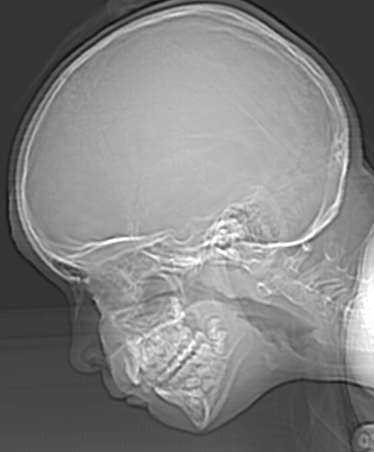
\includegraphics[width=0.2\textwidth]{ctskull-256.png} &
    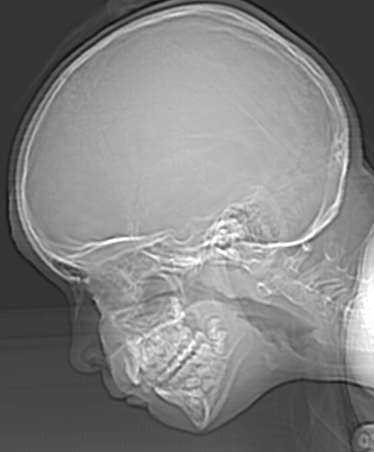
\includegraphics[width=0.2\textwidth]{ctskull-256.png} &
    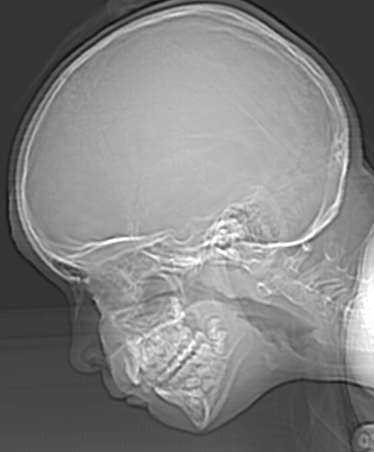
\includegraphics[width=0.2\textwidth]{ctskull-256.png} &
    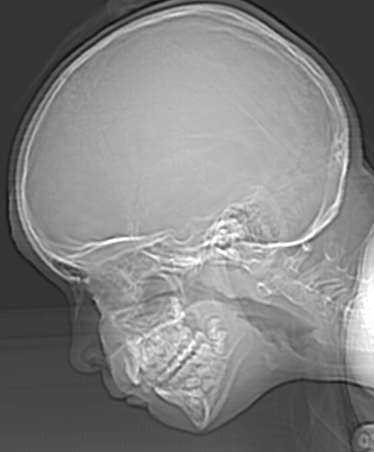
\includegraphics[width=0.2\textwidth]{ctskull-256.png}\\
    256 levels & 128 levels & 64 levels & 32 levels \\
    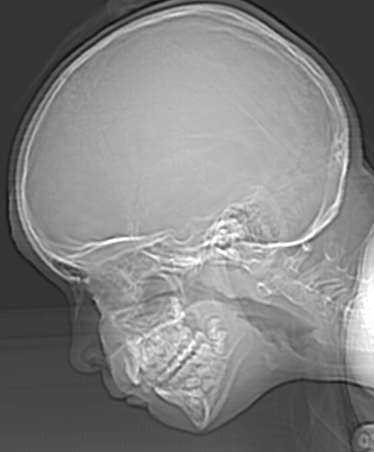
\includegraphics[width=0.2\textwidth]{ctskull-256.png} &
    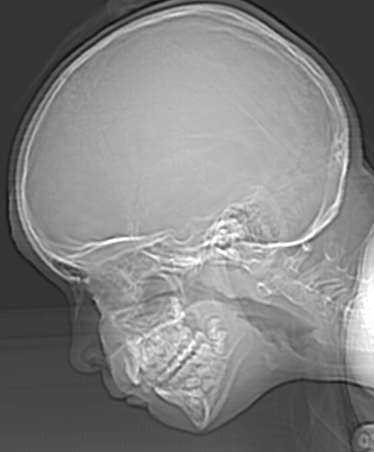
\includegraphics[width=0.2\textwidth]{ctskull-256.png} &
    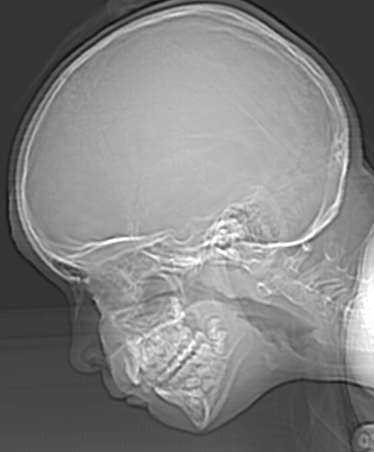
\includegraphics[width=0.2\textwidth]{ctskull-256.png} &
    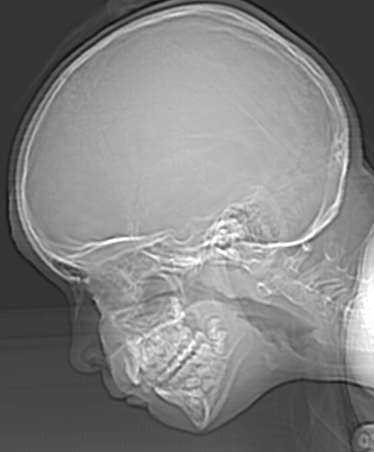
\includegraphics[width=0.2\textwidth]{ctskull-256.png}\\
    16 levels & 8 levels & 4 levels & 2 levels
\end{tabular}
\end{center}
\end{enumerate}


\exercise{Handing in}
\noindent When you're done, construct an archive file (zip, tgz, or
tar) which contains your report and Matlab files. Then hand it in
according to the instructions of the lab assistants.

\end{document}
